\chapter{可信机器学习基础}
\label{chap:trust-foundations}

上一部分已经建立了从样本判断总体风险的条件：固定假设空间、损失、抽样关系和比较基准后，有限样本泛化界给出这种推广的误差与失败概率。这里保证的是既定总体上的统计性质。把学到的模型交给实际系统使用，还需要确定这些性质能支持什么行动。

同一个预测结果可以触发不同处置，处置的后果也可能由不同的人承担。因此，从可学习性进入实际使用时，我们需要明确保证约束的是预测误差、概率校准、预测范围覆盖，还是模型与决策流程共同产生的行动损失。质询和复核的渠道、条件改变后的监测责任以及补救措施，也都属于使用判断所需的信息。

我们先看一个邮件分类器。它在测试集上的准确率为97\%，系统据此把可疑邮件放进可恢复文件夹，或者直接删除，这两种用法能否得到同样的支持？隔离误判还有找回的机会，永久删除却可能使收件人错过求职通知或丢失合同附件。模型的误判率即使有有限样本保证，也没有回答应当授予哪一种权限。

\term{可信机器学习}（trustworthy machine learning）围绕这一使用问题研究：模型和使用过程在什么条件下满足合理要求，哪些证据足以支持这些要求。可信性随任务、受影响者和使用范围而定。例如，概率预测可靠的模型仍可能泄露训练信息；抵御了某类攻击的模型仍可能对少数群体频繁出错。我们需要分别提出并检验这些主张，综合得分不能替代它们。

本部分着重讨论技术可信性，即模型、数据、算法和技术系统的证据能够支持哪些主张。这些证据可以供组织审批、法律合规和公共治理复核。部署权限、责任归属和风险接受则还要由有权主体结合领域规则，以及受影响者提出的影响证据、质询与补救需求来决定；单凭技术测试通过，无法完成这些判断。本部分的范围因而只是人工智能治理所需材料的一部分。

要回答邮件分类器可以承担多大决策范围，我们将先把使用情境转成明确要求，再判断证据支持的强度，最后说明结论何时失效、谁采取限制措施、如何恢复。系统属性用于选定可靠性、隐私等考察维度，规范要求把维度落到具体条件；证据与生命周期安排则使这些要求可以被论证、复核和持续使用。章末回顾相关研究的汇合，并借研究地图指出仍缺证据的问题。这套分析也将贯穿可靠性、鲁棒性、公平性、行为约束、可解释性、隐私和安全各章。

图~\ref{fig:trust-technical-scope}把上述技术证据放在同一使用情境中考察。交叉区域表示各方会讨论共同议题，不能据此推断一种判断包含另一种判断：技术检验通过，仍不足以推出部署合法、已经获准或得到公众认可。

\begin{figure*}[htbp]
  \centering
  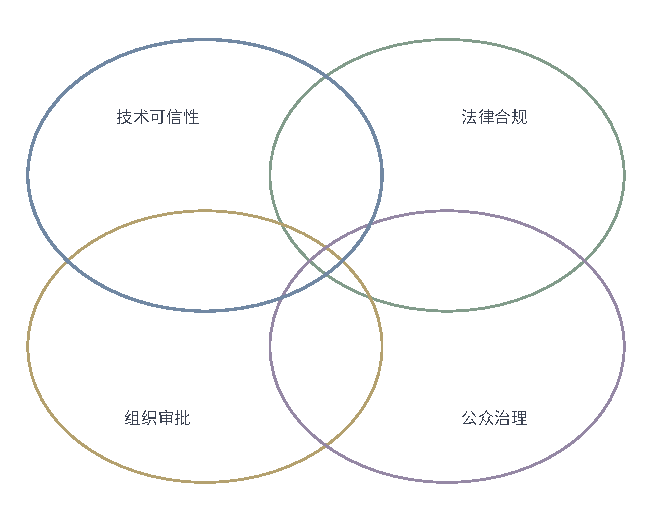
\includegraphics[width=111.404mm]{figures/03-foundations/03-trustworthiness/tikz/trust-technical-scope/figure.pdf}
  \caption{蓝色轮廓标出本书讨论的技术证据，其他区域表示法律合规、组织审批与公共治理。交叉处只示意共享议题；边界及面积不表示集合度量、逻辑包含或责任继承，各主体仍依自身要求判断。}
  \label{fig:trust-technical-scope}
\end{figure*}

\section{技术可信性的范围与三个层次}
\label{sec:trust-context}

邮件误拦的风险要沿着“预测—处置—后果”计算。确定后果后，我们还需要指出谁承受损失，以及哪些人和环境属于评价范围。前一项决定损失怎样计量，后一项限定这个损失结论能用于哪里；一个脱离这些信息的性能数值无法决定使用权限。

“可靠性”或“隐私”只是系统属性的名称，告诉我们要考察哪种性质。把属性写成规范要求时，还要给出受影响对象、评价单位、适用范围，以及允许的事件、阈值或程序条件。例如，邮件隔离要求可以约束误拦比例，而数据访问要求可以约束授权流程。这是分析的第一层。

第二层检查已有证据是否足以支持要求。理论结论要保留显式假设和量词，抽样检验要交代数据取得方式；压力测试、机制分析与人因评价则补充各自能够观察的失效。反证和剩余不确定性需要与有利结果一同记录，才能看清结论的强度。

第三层把结论带回运行过程：哪些条件改变会使主张失效，谁负责监测，触发后怎样限制使用、回退和恢复。技术材料提供这些判断所需的依据，有权主体再据此决定是否接受剩余风险和批准部署。

三层各有不能省略的职责。要求确定测试要支持什么行动，证据说明要求是否得到支持，生命周期条件限定证据何时继续有效。如果数据、模型、权限或用法已经改变，却仍沿用一次测试的结论，三层之间的联系就被切断。下面从邮件处置的后果建立第一项联系。

图~\ref{fig:trust-three-layers}同时标出提出要求、准备和复核证据、执行处置的角色。这些职责需要落实到实际授权记录；算法能够提供计算结果，却无法自行承担上述分工。

\begin{figure*}[htbp]
  \centering
  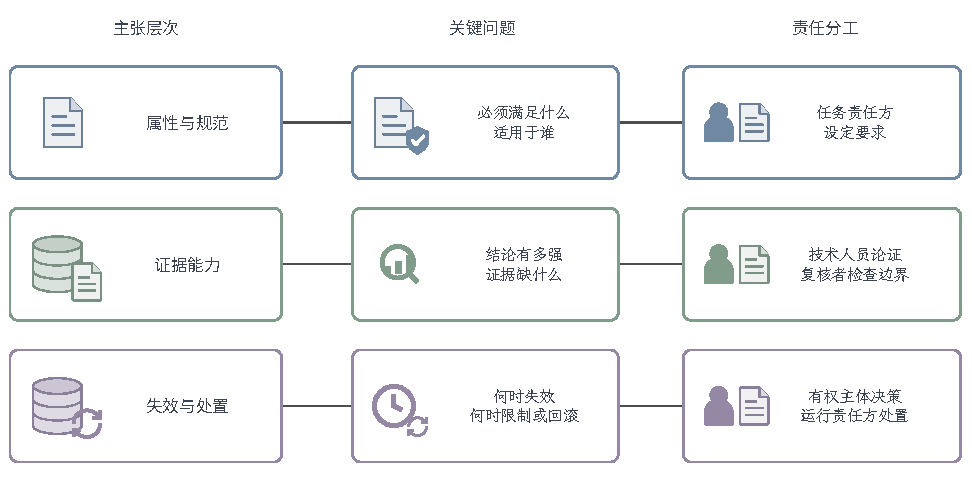
\includegraphics[width=164.600mm]{figures/03-foundations/03-trustworthiness/tikz/trust-three-layers/figure.pdf}
  \caption{要求、证据及失效处置构成可信主张的三个层次。系统属性选择考察维度，规范要求确定条件；证据限定结论强度；生命周期条件确定暂停沿用和响应。三行分别连接任务方的要求、技术论证与独立复核、有权主体的风险决定和运行方处置。横线只表示同层对应，教学分工仍需由真实授权与审批落实。}
  \label{fig:trust-three-layers}
\end{figure*}

\subsection{从预测结果到实际后果}

设一封邮件的输入为$\bm{x}$，模型输出为$f(\bm{x})$。系统还需通过决策规则$d$把输出变成行动$a=d(f(\bm{x}),\bm{x})$：例如根据垃圾邮件概率放行、隔离或转人工。我们可以保持$f$不变，只改变$d$，观察行动后果怎样改变。

为了给不同处置使用同一比较口径，记真实状态为$y$，采取行动$a$后的损失为$L(a,y)$。部署分布$\mathcal P$规定哪些邮件及状态进入评价，我们对这一分布取平均，得到系统的期望损失
\begin{equation}
 R_{\mathrm{sys}}(f,d)
 =\mathbb E_{(\bm{x},y)\sim\mathcal P}
 L\bigl(d(f(\bm{x}),\bm{x}),y\bigr).
 \label{eq:trust-system-risk}
\end{equation}
式中保留了模型、决策规则与数据分布三者。分类器的零一损失只区分预测是否错误，行动损失还区分误拦和漏放的后果。两种损失分别回答预测质量与使用代价问题，不能相互替换。

图~\ref{fig:trust-decision-consequences}保持预测不变，分别画出隔离和永久删除的行动链。我们要比较的是链条末端的后果，而不只是链条开始处的分类结果。

\begin{figure*}[!htb]
  \centering
  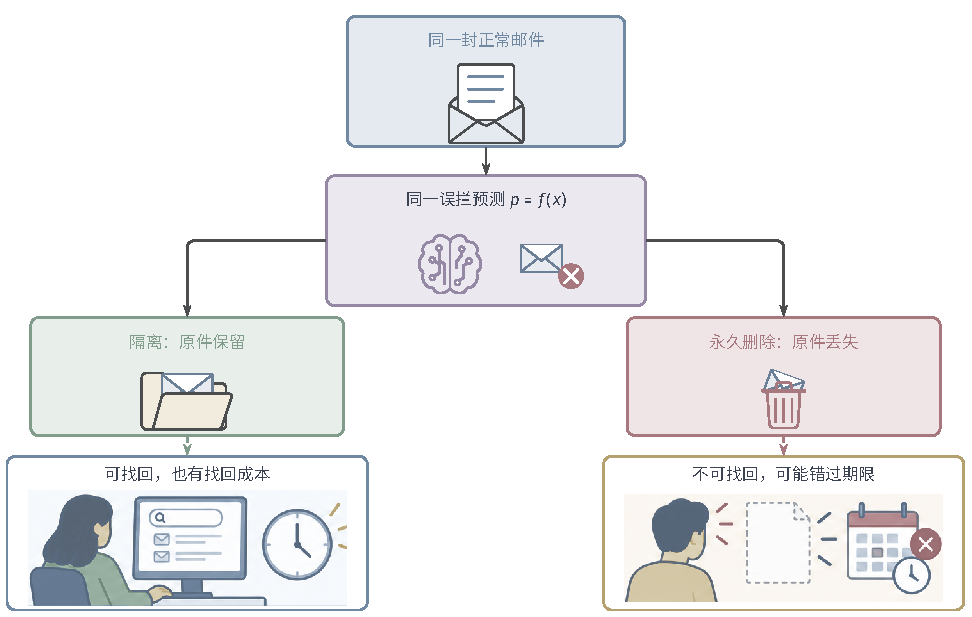
\includegraphics[width=164.600mm]{figures/03-foundations/03-trustworthiness/tikz/decision-consequences/figure.pdf}
  \caption{保持$p=f(\bm x)$不变，比较同一正常邮件误拦后的隔离与永久删除。左侧保留原件可供找回，右侧删除原件；末端收件人可能承担找回成本或错过期限。$L(a,y)$还需计入真实状态$y$、发现延误和恢复成本。情景为构造，保留原件并不保证及时找回。}
  \label{fig:trust-decision-consequences}
\end{figure*}

\begin{example}[准确率与行动损失]
\label{ex:trust-mail-cost}
在一个构造的1000封邮件测试集中，模型甲误拦10封正常邮件、漏放20封垃圾邮件，模型乙误拦2封正常邮件、漏放40封垃圾邮件。按正确封数计算，甲的准确率为97\%，乙为95.8\%。现在把每次误拦损失设为10、每次漏放损失设为1：甲产生的总损失为$10\times10+20=120$，乙为$2\times10+40=60$。同一测试集上，乙虽然正确率较低，却减少了在此损失设定下更昂贵的错误，因此总行动损失较低。比较结论仍限于这批样本和成本设定，不能单独决定使用权限。
\end{example}

这个例子借人为指定的代价说明，正确率的排序与行动损失的排序可以不同。真实邮件流程还要计入延误、申诉和恢复成本。隔离若能及时找回，可能比永久删除损失小；用户若一直没有发现误拦，保留原件也未必实现补救。评价因此要追踪完整流程。

知道不同错误的成本后，我们可以从损失推导处置阈值。这里比较邮件隔离和放行，按各行动在当前输入下的期望损失选择。设$p$为给定输入下邮件属于垃圾邮件的真实概率，误拦成本为$c_{\mathrm{fp}}>0$，漏放成本为$c_{\mathrm{fn}}>0$，正确处理暂不计成本。隔离只有遇到正常邮件才产生损失，其条件期望为$(1-p)c_{\mathrm{fp}}$；放行的条件期望为$pc_{\mathrm{fn}}$。选择损失较小的行动，隔离条件便是
\begin{equation}
 p>\frac{c_{\mathrm{fp}}}{c_{\mathrm{fp}}+c_{\mathrm{fn}}}.
 \label{eq:trust-cost-threshold}
\end{equation}
两项损失相等时，当前模型下的行动等价。误拦成本越高，隔离所需的概率越高，阈值因此不必是0.5（可参考\BookDefinitionRef{def:decision-conditional-risk-bayes-rule}{卷2《数学准备：概率、因果与决策》第6章“策略的价值与优化”第6.4.1节“单步价值下的行动选择”}）。实践中代入的是估计概率，决策质量便依赖估计质量。若干概率区间的平均预测与事件频率吻合，只给出分组证据，不能证明每个输入上的概率准确；第~\ref{chap:trust-reliability}章将展开这些区别和检验。

\begin{example}[增加复核选项后的决策]
\label{ex:trust-review-cost}
沿用教学成本$c_{\mathrm{fp}}=10$、$c_{\mathrm{fn}}=1$，再加入一个固定成本为0.2且能够无误确认标签的人工复核选项。隔离、放行和复核的候选损失分别为$10(1-p)$、$p$和0.2。比较三者，$p<0.2$时放行损失最小，$p>0.98$时隔离损失最小，中间的$0.2<p<0.98$则由复核占优；两个端点各有两种行动成本相等。复核区域来自成本比较，不需要模型额外预测一个“犹豫”类别。
\end{example}

无误复核使这项计算可以只用固定成本0.2。若人工也会出错，或者队列变长使等待成本增加，就要把相应后果计入第三项。进一步判断模型是否值得使用，还需在相同条件下比较完全人工处理、简单规则或较低权限的自动化；两个模型的准确率比较没有覆盖这些替代流程。

成本难以精确给定时，我们可以改变成本比，重复比较同一组可行方案的期望行动损失。由领域约束和有权主体预先声明的成本比区间限定分析范围：方案若只在窄区间占优，结论依赖较精确的成本判断；若在整个区间均比各替代方案损失低，结论对该项不确定性较不敏感。这里改变的是使用假设，区别于第~\ref{chap:trust-robustness}章的输入和环境变化。

式~\eqref{eq:trust-system-risk}还把真实状态$y$当成不随当前行动变化的对象，邮件类别通常可以采用这一建模。资源分配却可能不同：用分数决定谁参加培训后，培训本身会影响后续成绩。过去参加培训者中的预测准确率，无法直接说明把名额给其他人会带来什么收益。要比较这些行动，我们需要描述各候选行动下的可能结果，并取得额外观测或提出因果假设；历史行动下的成绩不能直接充当所有行动共用的$y$。这一区分将在第~\ref{chap:trust-fairness}章的长期干预分析中再次使用。

\subsection{风险的承担者与使用范围}

损失确定后，还要说明损失落在谁身上。购买、操作系统的人与受影响者可能不同：招聘筛选为用人方节省工作，却可能让求职者承担误拒。评价需要同时记录收益、错误负担以及发现和纠错的机会；开发者容易测量的指标未必覆盖这些影响。

同一种损失也会随语言、设备、时间、输入质量和用户群体而改变。部署范围中的“适用于某类输入”应当对应可检查条件，范围外输入则需要识别、限制使用或转交安排。环境变化怎样破坏原有规律，留待第~\ref{chap:trust-robustness}章分析。

把失效列入具体使用情境，还会发现预测以外的危害：答案正确却泄露隐私，完成指令却越过授权，或受外部内容诱导偏离任务。明确这些路径，才能选择相应保护。NIST人工智能风险管理框架也从使用情境识别、测量和管理风险；应用其原则时，仍须把要求落实到当前系统\scite{nist2023rmf}。

\section{系统属性与规范要求}
\label{sec:trust-requirements}

使用情境已经给出危害及承担者，接下来要把危害转成可判定要求。要求设定包括三个相连的工作：写清可观察的主张，检查遗漏的情境，再处理各项要求之间的支持或冲突。可观察事件把后果与行动规则连起来；只描述后果，无法测量改进，只优化一个没有行动含义的数值，也可能偏离使用目的。

\subsection{可信性要求的具体表达}

在邮件任务中，“可靠”可以具体约束自动隔离邮件中的正常邮件比例，也可以约束某一人群的预测区间覆盖率。两条要求的承载对象不同，需要分别声明评价单位、总体范围、错误事件和容许水平。这样才能判断一个测试究竟支持了哪条主张。

评价单位还决定风险怎样累积。以一次调用计量的失败率，不能直接作为用户一周全部调用的失败率；连续调用可以把很小的单次概率累积成较大的至少一次失败概率。多步任务因此要同时评价单步性质和最终结果。

有了评价单位，我们仍需选择要求的表达方式。平均行动损失适合比较可补偿的代价，发生概率、分组要求和授权访问等过程条件则可能要单独约束。设任务、模型供给、允许行动及权限边界确定了候选模型族$\mathcal F$与决策规则集合$\mathcal D$。在可量化要求下，可以选择满足约束且平均损失最小的一对模型与规则：
\begin{equation}
 \begin{aligned}
  \min_{\substack{f\in\mathcal F\\d\in\mathcal D}}\quad
  &R_{\mathrm{sys}}(f,d)\\
  \text{s.t.}\quad
  &G_j(f,d)\leq b_j,\quad j=1,\ldots,m.
 \end{aligned}
 \label{eq:trust-constrained-objective}
\end{equation}
$G_j$表示第$j$项要求的测量量，$b_j$给出其容许上限，$m$为要求数。先用约束排除不允许的方案，再按$R_{\mathrm{sys}}$比较剩余方案，这说明了最小化的用途。最小值写法要求可行集非空且最优解能够取得；否则应报告不可行或使用下确界。无法合理量化的程序条件仍需保留在公式之外，不能制造分数来代替它。

\subsection{可信性要求的完整性}

满足现有风险要求的模型可能不止一个，而且这些模型在部署关切上仍有差异。\term{欠规定性}（underspecification）描述的正是这种信息缺口：任务与评价条件足以让多个模型通过，却不足以区分其重要行为。判断时须预先指定训练域留出数据、指标和容差；候选模型可能同时达标，或指标差异落在容差内，却在新环境、子群体或压力情境中给出不同结果。D'Amour等在多种流程中展示了这一现象，提醒我们除检查单个模型是否过拟合，还要检查训练和评价条件能否筛选出所需模型\scite{damour2020underspecification}。

我们用一个构造邮件问题区分这两种缺口。若训练来源中内容特征$x_1$与页脚特征$x_2$始终相同，标签也等于两者，则只使用其中任一特征的分类器在同分布测试中都完全正确。增加同来源的测试邮件只能更准确地确认这种等价，无法决定部署时哪条规律会保持。若部署仅保留内容与标签的关系，两个候选的行为就分开了；此时所缺的是区分规律的新情境。

补充信息可以改变训练，也可以改变评价。训练端加入环境、结构约束或领域知识，评价端构造能够区分候选规律的测试；采用哪一种取决于部署中可获得什么信息。压力测试只验证了某个随机种子产生的模型时，结论也只属于该模型，不能转给其他种子重训的结果。

要求还可能漏掉同一标签内部的差异。\term{隐藏分层}（hidden stratification）指标签和评价分组未表示某些子类型，而它们的错误概率、损失、补救机会或行动规则不同；聚合后便看不见重要失败。Oakden-Rayner等的医学影像研究讨论了低频子类型、标注质量和伪相关引起的问题。由此需要检查标签是否充分描述任务差异，而不能把自动聚类形成的每个组都认定为有实际意义\scite{oakdenrayner2019hidden}。

“正常邮件”中的普通通知与有截止日期的合同便可能承担不同的误拦代价。我们可以根据后果提出候选切片，再核验样本质量和估计不确定性。错误分析发现的新切片用于诊断，独立确认才用于支持结论；反复搜索后找到的最差切片也可能只是抽样波动。环境切片和群体切片分别由鲁棒性与公平性两章展开，此处得到的共同结论是：没有被评价分组表示的要求，不能由总体指标代为满足。

\subsection{不同性质之间的联系与取舍}

要求完整性要覆盖几种不同对象。可靠性评价预测及不确定性是否有依据，鲁棒性评价输入和环境改变后的有效性，公平性评价机会、错误和负担的分配，目标对齐与行为约束评价学到的行为。可解释性提供理解和质疑行为的证据，隐私限制数据使用中的泄露，对抗安全则要求在主动操纵下保持相应边界。

同一处置会同时改变这些对象。例如，转人工可能降低自动处理部分的错误率，却减少自动处理量；隐私保护可能增加估计噪声；缩小工具权限可能减少损害，也可能阻碍完成任务。比较时需要沿用同一使用目标，报告收益及代价落在哪些指标和人群上。

加权综合分数还允许指标相互补偿，但某些要求并不允许这种交换。未经授权披露数据若被声明为不可接受，提高准确率不能抵消披露。式~\eqref{eq:trust-constrained-objective}据此把约束与优化目标分开。受影响者提供后果和补救需求，领域与法律规则给出外部边界，经授权责任主体在自己的权限内设定阈值、记录取舍并作有期限的风险接受。算法在给定要求下求解，风险接受也不能越过不可补偿约束。

\section{证据能支持什么结论}
\label{sec:trust-evidence}

明确要求之后，我们要判断证据能支持的强度，并检查证据怎样产生、如何保存以供复核。结论含义、检验设计与记录条件各自影响证据有效性；至于系统变化后能否继续沿用结论，下一节再讨论。

我们可以用一份\term{可信保证}（trustworthiness assurance）记录连接要求和证据。这里的保证是一项可逐条核对的论证，并非无条件承诺。记录包含十个字段：
\begin{enumerate}
  \item 使用情境与危害：任务、受影响者、评价单位和行动链；
  \item 规范要求：指标或程序约束的分母、阈值与适用范围；
  \item 显式假设：抽样、标签、权限、资源和替代方案等条件；
  \item 论证：保留量词和比较基准，解释条件怎样推出主张；
  \item 多源证据：理论、随机抽样、压力测试、机制分析、人因评价和监测；
  \item 反证与剩余不确定性：失败案例、未覆盖情境、估计误差和替代解释；
  \item 责任主体：证据准备、独立复核、监测、处置及外部决定的授权；
  \item 风险接受：有权主体在一定范围和期限内如何接受剩余风险；
  \item 失效触发：暂停旧结论的数据、模型、权限、流程变化或监测结果；
  \item 处置：降级、停用、回退、通知、补救、复验和重新开放。
\end{enumerate}
风险接受不由技术证明推出，主要由他人承担的损失也不能被默认为获准。失效来源进入情境、假设和触发项；主动攻击者存在时，还需记录其知识、权限、资源、目标及损害路径。

\subsection{理论保证与经验检验}

某个覆盖定理可能约束校准数据与未来样本的联合抽样，却没有约束每个固定输入的覆盖率。理论保证必须连同量词和假设一起使用，才知道它回答了哪一项要求。复核时因而要把数据生成、算法实现和评价对象逐项对照定理。

经验检验则在具体样本或攻击条件中观察系统行为。它可以发现现实与理论假设的偏差，也可比较尚无完整理论的方法。观察不到失败仍只是一项样本结果；我们先通过零次失败的计算看清它能支持多强的判断。

\begin{example}[零次失败的含义]
\label{ex:trust-zero-failures}
固定系统在$n$次独立同分布试验中的单次失败概率为$p$，整批零次失败的概率为$(1-p)^n$。把这个概率置为$\delta$并求解，可以得到零失败观测所对应的单侧置信上限
\[
 p_{\mathrm{up}}=1-\delta^{1/n}.
\]
取95\%置信水平，100次零失败的上限约2.95\%，1000次零失败约0.30\%。95\%属于构造上限的程序在重复抽样中的覆盖性质，不能解释成固定未知$p$有95\%后验概率低于上限。上述计算还依赖试验单位和抽样条件；若不断尝试，直到某批恰好零失败才报告，原来的置信解释不再成立。
\end{example}

\subsection{检验设计与证据有效性}

除了随机抽样，我们还可以按已声明的行为要求主动设计用例。\term{行为测试}（behavioral testing）把某种输入或变化应触发什么响应写成可执行检查。Ribeiro等的CheckList将语言能力与最小功能、保持不变、定向变化等测试结合，帮助把行为预期落实为用例，补充总准确率未直接检查的部分\scite{ribeiro2020checklist}。

对邮件系统，最小功能用例可以是一封简短且含义明确的会议通知；保持不变用例只改大小写或无关排版，仍要求放行；定向变化用例则在任务已把某类未经请求的推销认定为垃圾邮件后，逐步加入明确推销内容，观察分数方向。这些预期都要受任务语义约束。例如，诈骗警示引用了诈骗原文，并不等于在实施诈骗；一律拦截引用会暴露模型对意图的遗漏。

行为用例用于寻找规定机制中的缺陷，随机抽样则在抽样条件下估计总体风险。困难样本被有意大量纳入压力测试，其失败率不能直接充当部署失败率；普通随机样本中没有遇到低频缺陷，也不能代替针对性检查。样本的取得方式决定了结果的解释范围。

数据的用途同样会改变证据。模型选择和阈值调整若反复读取测试结果，测试集便参与了开发。最终评价需要另留未参与选择的数据，或采用处理重复选择的统计方法；第~\ref{sec:reliability-guarantee}节会给出有限候选程序的例子。

比较系统时，还需固定任务、样本、资源预算和评价口径。随机生成过程要记录生成次数、解码设置与选择规则；用一个系统多次生成后最好的结果对比另一个系统的首次结果，改变的不只是模型，也包括计算和选择机会。

人或模型给出的分数也是测量过程的一部分。我们需要核查判据、重复一致性及其与实际后果的关系：偏爱长答案的评判者可能提高冗长答案得分，而事实正确率没有增加。保存模型版本、数据来源、评价规则和运行条件，才能复核分数究竟表示什么。

\subsection{证据的记录与复核}

测试数值的适用条件往往藏在数据取得过程中。重复记录、标签来源、排除标准及预训练语料重合，都可能影响结果。Gebru等提出Datasheets for Datasets，随数据记录动机、组成、收集过程和推荐用途，以便使用者判断数据是否适合当前任务。这些说明限定数据条件，却不证明数据没有偏差\scite{gebru2021datasheets}。

模型层面也需要保存对应条件。Mitchell等的Model Cards记录预期用途、评价过程和相关群体或情境下的结果，使模型名称对应到具体版本、范围与证据。模型卡可以承载可信主张；卡片填写齐全而评价缺失时，主张仍缺证据\scite{mitchell2019modelcards}。

例如，模型卡报告较低的正常邮件误拦率，数据说明却显示样本只来自一种语言和一组用户。把两份记录对照，复核者便能识别另一种语言尚未获得支持。补做测试后，应更新该语言的覆盖范围和证据，单独改变模型版本号无法补上这个缺口。

复现也有不同范围。重跑同一程序核查计算和随机性；新增独立样本核查结论在重新抽样后的重复性；换环境核查外部适用性。三项依次改变的对象不同，结论不能互相推出。公开代码主要帮助重跑程序，后两项仍需合适数据和环境联系。

生成系统还要保存决定输出分布的过程：模型版本、系统提示、检索内容、工具权限、温度、重试次数和答案选择方式。若更新模型的同时增加重试，收益属于这套完整过程，不能全部归于模型能力。记录这些条件也为下一次重新验证确定了比较对象。

\section{失效、处置与生命周期条件}
\label{sec:trust-lifecycle}

证据已经说明要求得到何种支持，运行中仍要判断这些条件何时改变。生命周期安排记录参与者、环境或组件怎样使主张失效，谁在何种范围接受剩余风险，哪些观测触发限制使用，以及怎样恢复到可评价状态。受影响者的质询和补救需求是决策输入，不能转成由其独自审批；有权主体作决定，也仍要考虑这些输入与外部约束。这里提供审批、监测和复查所需的技术材料，不替组织设定法定职责。

\subsection{失效来源、责任主体与风险接受}

保证依赖的数据、标注、供应商、权限、人员负荷或组件状态，都可能发生变化。我们将这些破坏保证条件的因素称为失效来源，并沿“作用对象—影响路径—能否监测”记录它们。若有人主动选择变化以造成损害，还要进一步设定威胁模型，说明攻击者的知识、权限、资源和目标。

条件改变时，必须有人能够执行处置。\term{责任主体}（accountable role）指对某项保证决定或行动承担明确职责的角色；评价准备、独立复核、使用审批、运行监测和事故处置可以分开授权。笼统地写“项目组负责”，无法确定谁在触发后有权停用系统。\term{风险接受}（risk acceptance）则由有权主体在证据边界和剩余不确定性已知时，决定残余风险能否在特定范围与期限内承担。接受不等于风险消失，也不允许用收益抵消不可接受的约束违反。

\subsection{变更触发与组合后的重新验证}

把通过测试的组件接在一起，会出现单独测试没有评价的新关系。检索结果可能改变生成器的输入分布，重试可能增加泄露机会，告警过多可能使人工审核失效。组合后的验证因此要检查这些接口和依赖，不能只重跑原组件测试。

要避免条件改变后误用旧证据，主张应当带有\term{失效触发}（invalidation trigger），明确哪些数据变化、权限扩张、模型更新或监测结果使其暂停适用。触发项给出可依赖结论的期限和边界。组织的审批、发布与追责还属于治理流程，技术记录则至少要提供决策点、所需证据和触发条件。

组件错误的关系也会随组合进入评价。若同一垃圾邮件总体中两个检测器各漏检10\%，任一报警便拦截，则只有两个漏检事件独立时，共同漏检率才是1\%。如果两者采用相同表征并遗漏相同邮件，共同漏检可能仍为10\%。第二个检测器能否减少风险，取决于它增加了什么信息，结构上多设一层并不足以证明收益。

人工复核同样不能只按组件数量计算收益。复核者看到原件和只看到模型摘要，能获得的信息不同；摘要若已漏掉关键证据，确认步骤未必修正判断。人机协作的风险主张需要评价复核者所见信息、告警数量与行动时间等真实条件，第~\ref{sec:alignment-oversight}节将进一步讨论这些监督要求。

\subsection{失效处置与恢复}

失效触发之后，先限制损害，再保存定位证据，随后恢复到可重新评价的状态。暂停自动动作、降低权限、转人工、回退模型或隔离数据，应根据危害选择。已删除内容、已泄露信息与可撤销状态的恢复边界不同，不能统称为“回滚即可”。通知受影响者、纠正已有结果及保留日志的安排，也需服从隐私和访问约束。

重新开放需要针对触发原因与修复范围建立新证据。复验既检查已知失败是否重现，也检查修复是否影响正常任务、其他群体和相邻性质。责任主体据此重估剩余风险；证据不足时，继续限制使用或选用危害更小的流程。监测、处置和恢复由此进入保证的成立条件，而不只是部署后的附加措施。

\section{例子：邮件隔离的完整保证记录}
\label{sec:trust-mail-assurance}

我们把前面建立的要求、证据和生命周期条件合在一次邮件隔离验收中。以下模型、数据、阈值和结果均为构造值，用于说明怎样形成可判定的保证记录，不代表真实服务经验。验收固定模型$v_1$与概率修正程序$c_1$，范围为公司自有网关在批准后30日内接收的中英文文本邮件；加密正文、纯图像邮件和网关外导入邮件均转出自动处理范围。

误拦可能延误合同和求职通知，漏放可能暴露诈骗内容。记录据此排除永久删除权限，并将用户代表的延误及恢复需求、运行方的人工处理能力和适用规则交由经授权产品责任人审定。在授权范围内，责任人采用$c_{\mathrm{fp}}=10$、$c_{\mathrm{fn}}=1$、复核成本$0.2$这组教学值，再预先声明验收条件。本次验收批次的隔离比例至少30\%，用于确认该批次中自动化分担了足够处理量；误隔离与漏放上界分别限制延误和诈骗危害；恢复时延的经验95\%分位数不超过5分钟，最大值不超过10分钟。这些阈值来自规范设定，不能看完结果再反推。

$c_1$使用与验收集独立、来自同一声明总体的校准资料冻结。校准记录按预设概率区间保存样本量、平均预测与事件频率，偏差超出预设容差便触发失效。这支持分组概率语义，尚未证明每封邮件的$p=c_1(f(\bm x))$都是真实条件概率。用$10(1-p)$、$p$和$0.2$比较处置因而是一项建模近似，还要独立验收冻结后的规则。规则规定：$p<0.2$时放行，$0.2\leq p\leq0.98$时复核，$p>0.98$时可恢复隔离。

独立验收以单封邮件为抽样单位，从声明总体独立同分布抽取1000封邮件，其中正常600封、垃圾400封。两名评价人员按照预先冻结的标签规则独立标注，第三人裁决分歧。冻结的处置规则隔离362封，其中正常邮件2封；复核100封，其中正常70封；放行538封，其中垃圾邮件10封。

我们分别检查四项预设要求。验收批次的自动隔离比例应至少30\%；在隔离邮件中，正常邮件比例的单侧95\%二项Clopper--Pearson置信上界不超过2\%；在全部正常邮件中，误隔离比例的同类上界不超过1.5\%；在全部垃圾邮件中，漏放比例的同类上界不超过5\%。分母依次是全部邮件、隔离邮件、正常邮件和垃圾邮件，因此四个点估计分别为36.2\%、$2/362\approx0.55\%$、$2/600\approx0.33\%$、$10/400=2.5\%$。后三项置信上界约1.73\%、1.05\%和4.20\%，均达到各自阈值。这里的95\%分别属于每项上界程序，不是三项同时满足的95\%置信保证；需要同时保证时，须事先分配总体失败概率并重新计算各项上界。隔离比例的36.2\%只用于核对上述验收批次门槛，未建立部署总体隔离比例至少30\%的置信下界，也不把这一点估计写成部署保证。

补救还需独立演练。50次演练从点击“恢复”起计时，到邮件同时回到收件箱和搜索索引为止。按最近秩规则，第$\lceil0.95\times50\rceil=48$个次序统计量给出经验95\%分位数3分钟，最大值7分钟，分别低于5分钟和10分钟。它们描述这50次演练，尚未构成未来时延总体分位数的置信保证。

上述论证依赖几项条件：验收邮件与随后30日邮件满足声明的抽样关系，标签可信；$v_1$、$c_1$、成本和阈值在验收前固定；人工队列可用，隔离区与搜索索引支持恢复。行动损失用于构造三段处置，范围检查限定自动处理对象，误拦与漏放比例的单侧置信上界处理抽样不确定性，恢复演练检查补救路径。每项证据都有相应的职责。

为了补充总体计数，记录还按语言检查：中英文各500封，每组隔离181封并误拦1封。40项预先声明的压力测试分别检查合同与求职邮件、诈骗原文引用、无关排版变化和范围边界，每类10项，每项事先确定预期动作，本次均未失败。定向用例只覆盖已列情境，不能据此估计部署失败率或保证其他情境安全。

验收通过仍保留失效可能。漏放上界虽达到教学阈值，新模板、隐藏子类型、共同训练盲点和人工错误仍未被排除；低频重要邮件的区间可能较宽，也尚无上线监测结果。评价人员冻结数据、复核标签并计算上界，用户代表提供后果与补救需求，产品责任人按授权批准期限，运行人员监测、停用与回退，用户能够查看隔离并申请恢复。

在这些条件下，教学实例的产品责任人接受$v_1$在声明范围运行30日，权限仅限可恢复隔离。主动攻击和隐私并未获得这项验收的正面保证；外部安全或隐私检查若发现违反约束，准确率收益不能抵消违反，永久删除也仍不获接受。

触发项需要按影响范围执行。某封邮件超出输入范围，只把该请求转人工；模型、修正程序、阈值、标签规则或工具权限改变，则暂停整项保证。运行人员每7日按预先固定的纳入概率，从该周期到达且满足输入范围的邮件流中独立抽样；只有在周期内邮件可视为来自同一稳定分布、纳入决定与类别及预测结果独立时，才沿用二项Clopper--Pearson上界。若改为从已完成周期的有限邮件集合中不放回抽样，就应改用与有限总体设计匹配的区间，并把结论限于该周期。取得可靠标签后，重算三项错误比例的单侧95\%上界。标签尚未齐全时保留待审样本，不只保留易获标签或已成功处理的邮件；若无法为随机样本补齐可信标签，相关总体风险结论暂停沿用。这些逐期上界用于预设运行告警，单次95\%不能解释为所有时点与指标同时有效的95\%保证；需要这种保证时，应预先控制重复检验的总体错误概率或使用适用的序贯方法。任一上界超限、运行抽样中的隔离比例低于30\%这一预设告警线、人工队列不可用，或恢复时延的经验95\%分位数超过5分钟、最大值超过10分钟，均暂停自动隔离；这条告警线不是部署总体隔离比例的置信保证。

已经确认的外部安全或隐私告警也触发暂停，但这些告警不表示本项验收已经证明安全或隐私。暂停后，运行人员转人工、回退已验证版本、恢复误拦邮件并保留事件记录；评价人员补齐证据，有权责任主体重新接受后，系统再分阶段开放。

\section{可信研究如何扩展证据边界}
\label{sec:trust-research-content}

\subsection{研究路线的汇合}

本章的问题来自几条研究路线的汇合：统计预测与决策理论研究误差和行动，模式识别研究复杂输入中的有效性，信息安全限制信息与权限，人机交互和软件保障检查理解与运行过程。下面按使用链回顾这些联系，作为概念路线而非唯一编年史，教学上的衔接也不代表历史因果。各路线分别回答局部问题，把模型接入筛查、推荐、医疗和资源分配之后，还需共同说明输出怎样触发行动、后果影响谁、系统变化后证据是否继续有效。

概率预报提供了较早的一种评价对象。Brier分数比较报告概率与实际结果，作为损失时构成\term{适当评分规则}（proper scoring rule）：如实报告真实概率的期望分数不会高于其他报告\scite{brier1950}。这使评价从类别是否命中扩展到概率的质量。分类准确率相同，概率质量仍可不同；概率质量相同，成本和权限不同又会产生不同处置。本章据此将概率输出的含义与行动条件分开考察。

\Needspace{16\baselineskip}
概率被用于筛查、排序和分配后，平均预测误差之外还出现了新的要求：报告概率与事件频率是否吻合，不确定性能否指出困难输入，区间或集合是否覆盖目标。神经网络校准研究显示，分类改进不会自动使概率可靠；共形预测利用可交换样本的排序关系建立有限样本覆盖\scite{guo2017calibration,angelopoulos2022conformal}。可交换表示样本次序重排不改变联合分布，独立同分布是更强的常见充分条件。研究的问题由答对多少，延伸到如何表达尚不能确定的答案。

这一延伸仍要区分评价对象。二元事件校准比较报告同一概率的样本中事件的长期频率；多类别向量、类别条件和群体校准各需声明事件及条件。共形预测约束预测集合的覆盖事件，两者都不保证单个答案正确。集合始终很宽或系统频繁转人工也可能满足覆盖，因而还需同时报告集合大小、拒答比例和错误代价，评价它为决策提供了多少有用信息。

不确定性表达进一步进入处置：集合、区间或拒答信号可以触发补充信息、其他工具或人工接管。增加处置选项便改变了分母，自动处理部分错误率、全部请求覆盖率和转交成本要一同报告。选择性预测、序贯决策和人机协作将研究对象推进到带备选流程的完整决策程序。

由分组频率或联合抽样得到的结论，仍不能直接用于判定固定输入正确。高代价决策需要把总体、分母和随机来源写在保证中，并区分零失败观测、平均校准与每次决定的依据。风险控制、拒答和变化环境覆盖，分别继续处理这些保证未覆盖的条件。

\Needspace{10\baselineskip}
部署可能改变训练时的输入条件。常见损坏基准以噪声、模糊和天气等构造可重复压力，跨来源数据则按医院、时间、地理或设备划分环境\scite{hendrycks2019corruptions,koh2021wilds}。随机平滑等方法另为局部扰动提供认证\scite{cohen2019smoothing}。描述变化时，我们需要分别写来源和意图、训练与部署的统计关系、任务语义。自然与对抗变化都可能偏移分布，对手也可能保持或改变答案，不能把这些维度归成互斥类别。

固定损坏类型和强度，可以比较模型在同一压力下的退化；真实跨来源数据同时改变采集中的多个因素，更接近部署，却更难定位原因；局部认证则约束输入邻域中输出是否变化，尚未检验医院、时间或人群差异。基准、跨来源评价和认证因此提供不同的互补证据，分别支持重复比较、来源差异诊断和规定集合内反例的排除。

这些证据都要先确定任务要求如何随变化调整。设备、人口、规则或输入质量改变时，模型权重虽固定，风险却可能变化；某些输入变化应保持答案，某些新信息应改变答案，还有些已离开任务范围。鲁棒性若只要求稳定，就可能连有意义的信息也消除，因而必须先声明变化范围、幅度、对手与语义。

随机留出用于估计约定总体的平均风险，压力样本用于寻找困难情境，认证用于排除集合内的特定反例。它们的数值不可互换，却能够合起来确定失效位置和证据边界。分布外识别、领域泛化与持续适应再进一步研究变化识别、更新时机和旧版恢复。

\Needspace{12\baselineskip}
2010年代的算法公平研究把评价分到人群和个体。个体公平比较任务上相似者的处理，机会均等类标准在真实结果条件下比较错误或选择机会，反事实公平借因果模型研究群体属性改变后的预测\scite{dwork2012awareness,hardt2016opportunity,kusner2017counterfactual}。技术据此测量差异、揭示指标冲突和分析干预，与伦理、法律和公共政策中的规范问题连接；哪些差异合理、哪些利益不可补偿，仍需由有权主体决定。

上述标准的证据条件也不同：群体率依赖分组与标签，个体标准依赖任务相似性，反事实标准还依赖结构因果模型及允许保留的路径。满足某个统计等式并未同时证明个体受到保护或长期分配没有扩大差距。评价必须分别记录测量、规范选择、因果假设和动态影响。

分组审计保留身份、标签与选择过程的关系，才能观察不同人经历的后果。系统决定谁进入下一环节后，过去决策还可能改变标签可见性。公平分析因此需要继续追踪数据形成、阈值分配、拒答与复核负担，以及这些决定如何改变下一轮观测，不能只报告静态差距。

样本可以估计差异，却不能自行决定应保留哪些群体、优先避免哪种错误或容许多大差异。技术分析将指标冲突、不确定性和干预后果提供给有权主体，由其在规范边界内作选择。数值证据与数值的使用权限需要同时进入记录。

\Needspace{12\baselineskip}
当模型的计算无法直接读出时，解释研究转向局部行为、内部表示和训练来源。LIME用局部代理，积分梯度用基准路径，SHAP用联盟分配，分别解释预测变化\scite{ribeiro2016lime,sundararajan2017ig,lundberg2017shap}。评价还需区分忠实性、完整性、人的理解与实际判断收益\scite{doshivelez2017rigorous}。反事实解释和算法补救则再问哪些可行行动能够改变结果，将解释与交互、因果和决策支持连接起来。

这些方法各自带来验收条件。局部代理需指定区域与近似误差，路径归因需说明基准和路径，联盟分配需说明特征缺失怎样处理。人员实验要检查使用者能否在真实决策中发现错误，简化任务中完成得更快并不充分。解释若用于补救，还须约束可行动变量、成本与连带后果，输入表中可以改写的数值并不一定是现实行动。

线性模型、浅层树和规则的结构常能显露部分决策逻辑，而深层网络和大型集成把计算分散到大量参数中。后验解释为局部行为、路径或贡献分配提供近似，尚未恢复完整推理。解释图因此要结合保真检验、使用者和任务评价，才能说明它是否帮助发现与纠正真实错误。

开发者定位训练和模型问题，复核者判断一次决定的证据，受影响者则需要质疑和可执行改正，三者需要的信息可能不同。先规定使用者、任务与标准，再选择解释及人因、因果可行性评价，才能把解释接入审计和补救。

\Needspace{10\baselineskip}
数据保护又引入了另一种保证。差分隐私限制相邻数据集上输出分布的变化，约束单条数据增加的信息；成员推断与训练提取则表明模型接口也可能暴露参与事实或内容\scite{dwork2014privacy,shokri2017membership,carlini2021extraction}。形式分析必须明确邻接关系、保护单位、随机机制和组合，在定义范围内允许任意辅助信息；经验攻击则取决于查询数、已有知识与选择策略。未被形式定义保护的对象仍可能被推断，一次攻击失败也未排除更强攻击。

训练可把记录影响留在参数中，所以删除原始记录并不等于删除训练影响。分布式参与方还可能分别观察数据、梯度、聚合和更新，重复查询也可累积攻击证据；保护范围因此需要覆盖训练、通信与发布接口。差分隐私预算按对应定理组合再次访问数据或多次数据依赖发布，对同一已发布私有结果的纯后处理或重复展示不自动追加预算。形式保证和经验攻击都须声明保护单位、组合方式、实现条件及效用代价由谁承担。

\Needspace{20\baselineskip}
对抗样本说明，普通测试中预测正确仍可能在输入邻域内找到失败；投毒、后门和模型提取又把攻击面扩到训练材料、供应链与查询接口\scite{szegedy2014intriguing,goodfellow2015adversarial,gu2017badnets,tramer2016stealing}。隐私研究中的统计推断与密码协议、安全研究中的威胁建模与鲁棒优化，都需要明示保护对象、观察能力和资源预算。

攻击阶段决定需要检查哪个环节：推理扰动作用于测试输入，投毒改写训练材料，后门在触发条件下激活隐藏行为，模型提取利用接口结果恢复功能或参数信息。固定脚本下防御有效，仍可能来自梯度遮蔽或评测盲区。允许攻击者根据防御调整搜索，并区分搜索失败与形式不可达，才能限定安全结论。

主动对手会观察系统并选择有利输入或时机，困难情境的出现方式因而不同于自然抽样。安全评价要记录知识、权限、查询预算和最终损害，固定攻击样本不能代表整个攻击空间。检索、插件和工具的接入还把威胁扩到供应链、权限与执行器，模型评价需要与软件安全的纵深防御和事故响应共同使用。

\Needspace{20\baselineskip}
开放任务中的人类反馈将行为而非固定标签作为学习对象。行为片段比较用于奖励学习，指令跟随进一步采用示范、奖励模型与策略优化\scite{christiano2017,ouyang2022instructgpt}。人的判断变成可优化信号后，反馈覆盖、奖励外推和监督能力都可能成为新的误差来源：样本漏掉部署行为，策略变化使奖励外推失准，较弱监督者也可能漏看更强模型的隐蔽错误。

监督者因此不仅给答案，还比较结果、声明原则、检查过程或评价长期后果；模型优化这些代理时，可能利用协议没有预见的行为。分析需要区分能力不足、目标欠完整、监督信息不足和新情境下约束失效。对齐工作贯穿目标形成、反馈、更新、监控及执行权限，单独增加训练后过滤无法覆盖这条链。

交互还延长了后果的出现时间。单次回答的错误可能立即可见，多步计划的早期偏离却可能到数次工具调用之后才造成损害；模型也会针对监督规则调整行为。静态用例不足以代表这段过程，监督和监控本身可能被规避。任务分解、可扩展监督、过程评价和权限隔离，分别处理人无法全面理解、核验或及时阻断的困难。

\Needspace{18\baselineskip}
数据集说明书、模型卡和风险管理框架把用途、版本、责任与生命周期保存在结果旁边\scite{gebru2021datasheets,mitchell2019modelcards,nist2023rmf}。这些工作为同一使用过程组织不同领域的证据：统计与优化判断性能，因果和交互判断后果与人的使用，信息安全、软件保障和治理判断运行边界。

保存来源、版本、用途、分组结果和限制，才能在环境改变后复查旧结论。文档的用途是恢复判断上下文，风险管理还要确定风险接受、监测和处置角色，以及限制权限、恢复状态和重新验收的流程。

一次发布记录还不够处理后续变化。权重、训练数据、提示、检索库、阈值和接口改变，都可能破坏原检验条件。版本追踪、变更评审、事故响应与恢复演练，使记录能够回答更新后哪些结论仍有效，并把重新验证纳入保证。

基础模型可以产生措辞不同而语义相同的答案，智能体还会检索、调用工具和改变持久状态。固定标签、单次预测、静态模型的评价范围因而需要扩展到开放语义、完整生成程序、连续交互与组件组合。分析沿数据、参数、上下文、输出和行动追踪信息，才能覆盖新的使用过程。

这一过程也连接了原本分别评价的性质：检索既提供事实证据，也可能带来注入；拒答减少错误，却可能集中等待和复核负担；解释有助审计，却也可能泄露信息或迎合检查器。需要研究证据的组合、冲突和共同失效，单独提高各项分数尚未回答系统问题。

以上路线从平均误差扩到概率和拒答，从同分布测试扩到变化与攻击，从总体指标扩到人群、个体和补救，再从静态模型扩到持续更新的系统。扩展增加了旧证据尚未覆盖的使用条件，原来的准确率等问题仍保留，只需连同行动损失、承担者、威胁和生命周期解释。下一小节集中研究这些联系中尚缺的证据。

\subsection{当前前沿}

图~\ref{fig:trust-research-problems-map}按三层组织“系统何时可以被依赖”的研究。第一层分成要求与影响、证据与行为、防护与治理；第二层分别展开要求操作化、未知识别与转交、风险收益与负担分配、变化适应与恢复、解释审计与补救、目标监督与权限、隐私安全与行动保护、联合保证与持续验证八个问题。第三层为其中五项列出代表课题，未列示例的问题并不表示已经解决。下面五组方向跨越这些问题，并不与第二层逐一对应。

\begin{figure*}[htbp]
  \centering
  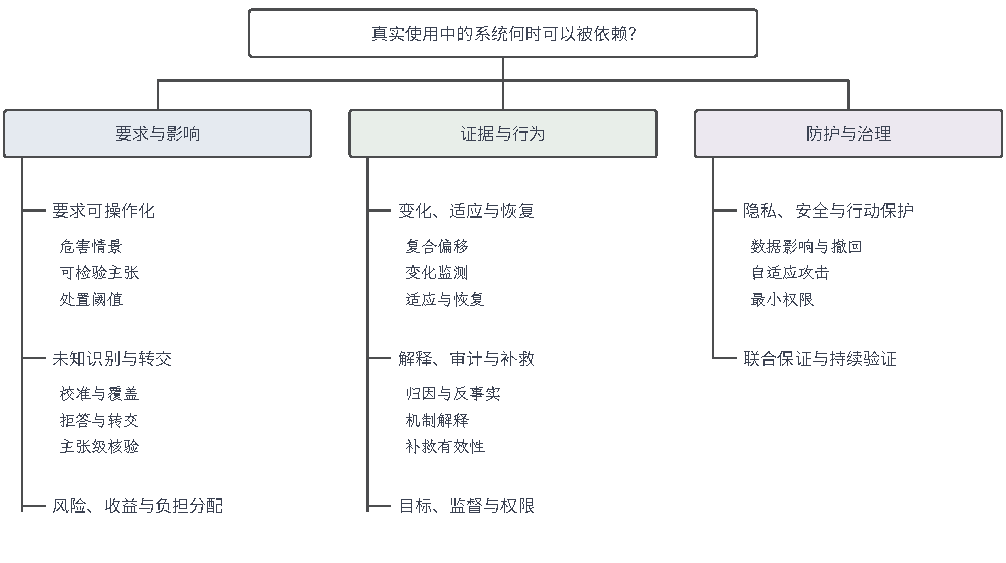
\includegraphics[width=164.600mm]{figures/03-foundations/03-trustworthiness/tikz/trustworthiness-map/figure.pdf}
  \caption{研究地图由使用问题向下展开：三组判断领域连接八项问题，其中五项列出危害情境、覆盖、复合偏移、机制解释、自适应攻击等十五项课题。连接线表示领域、问题和课题的组织层次，排列不表示因果或先后顺序。其余三个问题仅是未列示例。}
    \label{fig:trust-research-problems-map}

\end{figure*}

\Needspace{22\baselineskip}
\paragraph{开放任务的要求表达与可靠性控制}

开放生成与智能体任务需要评价事实主张、检索依据、工具调用、交互轨迹和状态变化，单个标签已不能覆盖这些对象。行为测试将预期转为用例，并利用失败发现遗漏\scite{ribeiro2020checklist}。但用例仍限于已经识别的情境。自动扩充数量若只改变表面形式，也不会补齐语义、权限或长期后果的边界。

可靠性于是要从整段得分追踪到单条主张、证据来源与行动风险。生成任务的共形扩展仍需先定义校准单元、覆盖对象、错误事件、集合构造与可交换等条件，才能解释其覆盖；覆盖本身没有核验事实\scite{angelopoulos2022conformal,loaizaganem2026confgen}。\term{语义熵}（semantic entropy）把含义相近的不同措辞合并，计算重复生成在语义上的分歧\scite{farquhar2024semantic}。两者衡量的对象不同，也都会遇到稳定复述同一错误、检索或筛选改变分布、生成器与验证器共享盲点等困难。

拒答、集合和人工转交将这些信号变成行动，却同时改变覆盖率、延迟和群体负担。研究需要把自动处理风险、拒答分布、备选流程容量及多轮选择的风险累积合起来约束。“不知道”的处置只有可以执行和复核、又没有简单把风险转给人工或特定人群，才支持使用判断。

\Needspace{22\baselineskip}
\paragraph{组合变化与长期分配后果}

现实部署往往同时改变设备、语言、人群、时间与策略，单因素扰动无法说明相互作用。跨来源数据展示复合偏移中的性能差异；脑电图（electroencephalography, EEG）基础模型的一项研究比较多个预训练模型、下游任务和数据集上的测试时适应，发现不同模型—任务组合的变化方向并不一致；在该研究的部分组合上，梯度式适应相对未适应基线的指定下游指标下降\scite{koh2021wilds,lee2026neuroadapt}。标签延迟或缺失时，研究还需判断观测外观改变是否已经影响风险，以及哪些原证据继续有效。

风险变化也改变人的经历：错误、等待和复核可能重新分配。机会均等与反事实标准使用不同标签和因果条件\scite{hardt2016opportunity,kusner2017counterfactual}。资源分配、拒绝与推荐又会改变下一轮可见数据。干预后群体差距受模型、行为响应和资源限制共同影响，静态差距因而不足以代表长期效果。

联合评价可以使用预设时间窗口，除平均风险外，记录风险最高或约束余量最低的时段、恢复到阈值的时间和更新后既有任务的回归结果。拒答、主动标注和人工处理负担也需按承担者记录。这样的时间轴把鲁棒性、公平性和服务流程连起来，检查收益是否将风险转移到别的环境、人群或测量范围之外。

\Needspace{22\baselineskip}
\paragraph{可扩展监督、机制解释与审计}

任务变长或变复杂后，人的示范、偏好与原则未必覆盖策略访问的行为，奖励模型可能外推失准，评价者也可能共有盲点\scite{christiano2017,ouyang2022instructgpt}。任务分解、过程反馈和弱到强监督试图扩大可用信息；较弱监督者仍可能看不出隐蔽错误，过程记录也可能偏离实际计算。这是扩大监督时需要同时保留的边界。

\term{可监控性}（monitorability）把监督困难写成可检验问题：在声明观察通道与监控能力下，能否以预设漏报、误报或发现概率识别行为、权限偏离\scite{burns2023weaktostrong,guan2026monitorability}。参与优化的监控器可能被规避，共享数据、架构或提示的检查者也可能相关出错。因此需要研究独立监督、随机审计、保留验收任务和抗规避监控，而不只测静态准确率。

稀疏特征分解等机制解释为内部状态提供观察入口\scite{bricken2023monosemanticity}。一个方向能够命名，还未说明任务计算因果依赖它；模型证据也要接到工具轨迹、权限与状态变化。只有支持发现错误、定位干预或实际补救的解释，才为可信使用增加了证据。

\Needspace{24\baselineskip}
\paragraph{隐私、安全与智能体行动}

隐私评价沿数据、参数、输出和参与方追踪信息。差分隐私约束保护单位对输出分布的额外影响，成员推断和训练提取检验接口泄露\scite{dwork2014privacy,carlini2021extraction}。前者需要保护单位、机制及数据访问和发布的组合，固定私有输出的纯后处理不自动新增预算；后者需要外部知识、查询数和选择策略。两者还要检查原件、参数、检索索引、缓存和审计副本中的信息残留，一次经验攻击失败并不能代替形式保证。

检索、长期记忆与工具使外部数据也可能影响控制。间接提示注入通过检索内容改变系统行为\scite{greshake2023indirect}。来源签名只能确认身份，不能保证内容安全；仅做输入过滤，仍未在执行端约束可调用工具的类型、权限和预算。威胁模型要覆盖供应链、接口与执行器，并允许对手依据防御反馈调整策略。

工具执行使损害进入持久状态。动态评测同时考察正常任务、有用第三方指令与恶意操纵，以测量安全和过度防御的取舍\scite{li2026agentdyn}。评价应区分文字改变、调用形成、实际执行及状态可恢复性，并检查突破后的恢复。自适应攻击、多组件供应链与端到端损害评估由此成为研究对象，防护仍需保留正常任务的可用性。

\Needspace{22\baselineskip}
\paragraph{联合保证与持续验证}

组件组合需要新的保证：检索器可能交出敏感信息，生成器可能给出正确调用却使用过大权限，低错误率组件也可能在同一输入上同时失败。保证案例与结构化证据图可以追踪主张在接口间的传递，但错误相关性与要求冲突仍需显式分析。简单加总、相乘或加权，会漏掉依赖和不可补偿约束。

持续使用还要连接记录与真实版本。说明书、模型卡和风险框架保存来源、用途、分组结果、限制及责任\scite{gebru2021datasheets,mitchell2019modelcards,nist2023rmf}。若记录未接入监测和变更流程，更新后便无法复核。权重、提示、检索、阈值、权限或人工流程任一变化，都可能要求重新判断证据。

为主张设期限与触发条件，再用线上监测、分阶段开放、回归检查和恢复演练控制变化，可以把保证维持在运行过程中。标签延迟、严重低频事件、版本并存与监测器失效仍是困难。研究要维护的是明确范围、可复核证据以及可发现、可处置的失效条件，永久标签无法承担这项职责。

\section{本章小结}
\label{sec:trust-foundations-summary}

回到章首，97\%准确率尚不能支持永久删除。要求层先限定自动处理范围、错误分母与不可补偿条件，证据层再说明独立样本、压力用例和机制检查支持了什么，生命周期层确定停用、恢复和风险接受职责。邮件实例据此只允许有条件的可恢复隔离。其2\%阈值约束隔离邮件中的正常比例，区别于全部正常邮件的误隔离率和全部垃圾邮件的漏放率。这三个分母分别界定三项错误率；每项规范阈值和置信上界都须按自己的分母解释，不能互换。

对预测与拒答的证据归入可靠性，对变化后有效性的证据归入鲁棒性，对机会、错误和负担的证据归入公平性。行为边界、理解与质疑、信息保护和主动攻击则分别由对齐、可解释性、隐私与安全补充。它们可以支持同一次使用判断，但一项改进没有替其他要求提供证明。

基础模型和智能体将这种判断扩到开放生成、多次调用和完整行动链。已有理论界、测试和干预分别解决了局部问题，组合变化、监督不足、自适应攻击与版本过期仍会破坏证据联系。评价需要沿使用过程保留这些剩余条件。

技术可信性因此形成一组带范围、证据和处置条件的主张。主张说明系统何时达到要求、哪里仍有不确定性，供审批和复查使用；职责安排、法律判断以及受影响者参与的治理决定，还需由相应主体作出。

\paragraph{延伸阅读}

继续阅读NIST人工智能风险管理框架时，可以沿本章情境把测量、风险处置、责任与触发条件对应起来，使框架中的原则转为具体记录\scite{nist2023rmf}。

数据集说明书与模型卡分别补充数据的动机、组成、采集条件，以及模型用途和分组评价。二者有助于限定记录的证据范围，仍要由实际测试支持其中的主张\scite{gebru2021datasheets,mitchell2019modelcards}。
